%\documentclass[10pt]{beamer}
%\usefonttheme[onlylarge]{structurebold}

\documentclass[handout]{beamer}
\usefonttheme[onlylarge]{structurebold}
  \usepackage{pgfpages}
\mode<handout>
\pgfpagesuselayout{4 on 1}[letterpaper,border shrink=5mm]

\hypersetup{
  bookmarks = false,
  colorlinks,
  citecolor = red,
  linkcolor=blue,
  urlcolor=blue,
  pdfpagemode=none,
  pdfstartview={Fit},
  pdftitle={},
  pdfauthor={Michael E. Waugh},
  pdfkeywords={} }
  \setbeamertemplate{navigation symbols}{}

\mode<presentation> {
  \usetheme{boxes}
  % or ...

  \setbeamercovered{transparent}
  % or whatever (possibly just delete it)
}

\setbeamertemplate{itemize subitem}[circle]
\setbeamerfont{frametitle}{size= \large}
\setbeamerfont{ framesubtitle }{size = \footnotesize}
\setbeamertemplate{frametitle}
{
\medskip
\smallskip
{\textsf{\underline{\insertframetitle\phantom{))))))))}}}}}


\usepackage[english]{babel}
\usepackage{wasysym}

\addfootbox{}{\hspace{5cm}\tiny {International Trade---Economics of Global Business, Revised: \today}}%

\title[NYU Stern] % (optional, use only with long paper titles)
{\Large International Trade}

\author[Michael Waugh] % (optional, use only with lots of authors)
{\bf{\Large}}%

\date[] % (optional)

\subject{Talks}

\begin{document}

\begin{frame}
  \titlepage
\end{frame}

%%%%%%%%%%%%%%%%%%%%%%%%%%%%%%%%%%%%%%%%%%%%%%%%%%%%%%%%%%%%%%%%%%%%%%%%%%%%%%%%%%%%%%%%%%%%%%%%%
%%%%%%%%%%%%%%%%%%%%%%%%%%%%%%%%%%%%%%%%%%%%%%%%%%%%%%%%%%%%%%%%%%%%%%%%%%%%%%%%%%%%%%%%%%%%%%%
\begin{frame}[t]
\frametitle{The Plan}
\bigskip
\begin{itemize}
\item Logic of trade
\bigskip
\item Develop Ricardian model of trade. Today\ldots
\begin{itemize}
\medskip
\item Opportunity cost and production possibilities.
\medskip
\item No trade equilibrium.
\medskip
\end{itemize}
\end{itemize}
\end{frame}

%%%%%%%%%%%%%%%%%%%%%%%%%%%%%%%%%%%%%%%%%%%%%%%%%%%%%%%%%%%%%%%%%%%%%%%%%%%%%%%%%%%%%%%%%%%%%%%%
%%%%%%%%%%%%%%%%%%%%%%%%%%%%%%%%%%%%%%%%%%%%%%%%%%%%%%%%%%%%%%%%%%%%%%%%%%%%%%%%%%%%%%%%%%%%%%%%

\begin{frame}[t]
\frametitle{The Logic of Trade}
\bigskip
\begin{itemize}
\item Voluntary exchange is ``win-win''
\begin{itemize}
\medskip
\item Suppose two people or firms value a product or asset differently
\medskip
\item Trade can benefit both
\end{itemize}
\bigskip
\item Example in labor markets:
\begin{itemize}
\medskip
\item You value your time at 50 an hour
\medskip
\item A firm values your time at 60 an hour
\medskip
\item At what price does trade take place?
\medskip
\item Who wins?
\end{itemize}
\end{itemize}
\bigskip
\end{frame}

%%%%%%%%%%%%%%%%%%%%%%%%%%%%%%%%%%%%%%%%%%%%%%%%%%%%%%%%%%%%%%%%%%%%%%%%%%%%%%%%%%%%%%%%%%%%%%%%
%%%%%%%%%%%%%%%%%%%%%%%%%%%%%%%%%%%%%%%%%%%%%%%%%%%%%%%%%%%%%%%%%%%%%%%%%%%%%%%%%%%%%%%%%%%%%%%%

\begin{frame}[t]
\frametitle{The Logic of Trade}
\bigskip
\begin{itemize}
\item Voluntary exchange is ``win-win''
\begin{itemize}
\medskip
\item Suppose two people or firms value a product or asset differently
\medskip
\item Trade can benefit both
\end{itemize}
\bigskip
\item Example in reality:
\begin{itemize}
\medskip
\item Green Bay Packers, Summer 08, 2 good quarterbacks
\medskip
\item NY Jets, none
\medskip
\item Solution:  trade!
\end{itemize}
\end{itemize}
\bigskip
\end{frame}

%%%%%%%%%%%%%%%%%%%%%%%%%%%%%%%%%%%%%%%%%%%%%%%%%%%%%%%%%%%%%%%%%%%%%%%%%%%%%%%%%%%%%%%%%%%%%%%%
%%%%%%%%%%%%%%%%%%%%%%%%%%%%%%%%%%%%%%%%%%%%%%%%%%%%%%%%%%%%%%%%%%%%%%%%%%%%%%%%%%%%%%%%%%%%%%%%

\begin{frame}[t]
\frametitle{The Logic of Trade}
\bigskip
\begin{itemize}
\item Voluntary exchange is ``win-win''
\begin{itemize}
\medskip
\item Suppose two people or firms value a product or asset differently
\medskip
\item Trade can benefit both
\end{itemize}
\bigskip
\item The price often depends on who has the most bargaining power. Consider this game
\begin{itemize}
\medskip
\item We have 100 dollars. Make me an offer on how to split 100 dollars.
\medskip
\item If I agree, we get to keep it. If not 100 dollars is destroyed.
\medskip
\item What offers would money not be destroyed?
\medskip
\item What is the ``Nash equilibrium'' outcome?
\end{itemize}
\end{itemize}
\bigskip
\end{frame}

%%%%%%%%%%%%%%%%%%%%%%%%%%%%%%%%%%%%%%%%%%%%%%%%%%%%%%%%%%%%%%%%%%%%%%%%%%%%%%%%%%%%%%%%%%%%%%%
%%%%%%%%%%%%%%%%%%%%%%%%%%%%%%%%%%%%%%%%%%%%%%%%%%%%%%%%%%%%%%%%%%%%%%%%%%%%%%%%%%%%%%%%%%%%%%%

\begin{frame}[t]
\frametitle{Reasons for International Trade}
\begin{itemize}
\bigskip
\item Relative costs of production, i.e. \textbf{comparative advantage}, rationalize international trade patterns.
\bigskip
\item What shapes a country's comparative advantage\ldots
\begin{itemize}
\bigskip
\item Technology, productivity of workers (absolute advantage).
\bigskip
\item proximity,
\bigskip
\item resources.
\end{itemize}
\end{itemize}
\bigskip
\end{frame}

%%%%%%%%%%%%%%%%%%%%%%%%%%%%%%%%%%%%%%%%%%%%%%%%%%%%%%%%%%%%%%%%%%%%%%%%%%%%%%%%%%%%%%%%%%%%%%%%
%%%%%%%%%%%%%%%%%%%%%%%%%%%%%%%%%%%%%%%%%%%%%%%%%%%%%%%%%%%%%%%%%%%%%%%%%%%%%%%%%%%%%%%%%%%%%%%%

\begin{frame}[t]
\frametitle{Ricardo's Model of Trade}
\bigskip
\begin{itemize}
\item David Ricardo, 1817
\begin{itemize}
\medskip
\item Two goods, countries have fixed productivity at producing them
\medskip
\item In free trade: each country produces one good
\end{itemize}
\bigskip
\item Key concept---comparative advantage
\begin{itemize}
\medskip
\item Each country should produce the good at which it is \begin{alertenv}{comparatively}\end{alertenv} the most productive.
\medskip
\end{itemize}
\end{itemize}
\bigskip
\end{frame}

%%%%%%%%%%%%%%%%%%%%%%%%%%%%%%%%%%%%%%%%%%%%%%%%%%%%%%%%%%%%%%%%%%%%%%%%%%%%%%%%%%%%%%%%%%%%%%%%
%%%%%%%%%%%%%%%%%%%%%%%%%%%%%%%%%%%%%%%%%%%%%%%%%%%%%%%%%%%%%%%%%%%%%%%%%%%%%%%%%%%%%%%%%%%%%%%%

\begin{frame}[t]
\frametitle{Ricardo's Model}
\bigskip
\begin{itemize}
\item Two countries (Home, Foreign), two goods (cloth, wheat), one input (labor)
\bigskip
\item Labor is mobile across sectors.
\bigskip
\item Constant marginal products of labor (MPL):
\end{itemize}
\bigskip
\begin{table}[t]
\begin{center}
\begin{tabular}{lccc}%
\vspace{-0.6cm}\\
\hline%
\hline
\vspace{-.4cm}       &\multicolumn{3}{c}{}\\
                     & Cloth  & Wheat  &  Labor \\%
\vspace{-.4cm}       &\multicolumn{3}{c}{}\\
\hline%
\vspace{-.4cm}       &\multicolumn{3}{c}{}\\
Home                 &   2    &   4     &   25  \\
Foreign              &    1    &    1     &   100  \\
\vspace{-.4cm}       &\multicolumn{3}{c}{}\\
\hline
\end{tabular}
\end{center}
\end{table}
\end{frame}

%%%%%%%%%%%%%%%%%%%%%%%%%%%%%%%%%%%%%%%%%%%%%%%%%%%%%%%%%%%%%%%%%%%%%%%%%%%%%%%%%%%%%%%%%%%%%%%%
%%%%%%%%%%%%%%%%%%%%%%%%%%%%%%%%%%%%%%%%%%%%%%%%%%%%%%%%%%%%%%%%%%%%%%%%%%%%%%%%%%%%%%%%%%%%%%%%


\begin{frame}[t]
\frametitle{Opportunity Cost}
\bigskip
\begin{itemize}
\item Opportunity cost: What you forgo when making a choice
\begin{itemize}
\medskip
\item This context, cloth you give up to make one more unit of wheat
\end{itemize}
\bigskip
\item For the Home
\begin{itemize}
\medskip
\item 1 wheat takes 1/4 units of labor
\medskip
\item 1/4 units of labor could make 1/4$\times2 = 1/2$ cloth
\medskip
\item Opportunity cost of 1 wheat is 1/2 cloth
\end{itemize}
\end{itemize}
\bigskip
\begin{table}[t]
\begin{center}
\begin{tabular}{lccc}%
\vspace{-0.6cm}\\
\hline%
\hline
\vspace{-.4cm}       &\multicolumn{3}{c}{}\\
                     & Cloth  & Wheat  &  Labor \\%
\vspace{-.4cm}       &\multicolumn{3}{c}{}\\
\hline%
\vspace{-.4cm}       &\multicolumn{3}{c}{}\\
Home                 &   2    &   4     &   25  \\
Foreign              &    1    &    1     &   100  \\
\vspace{-.4cm}       &\multicolumn{3}{c}{}\\
\hline
\end{tabular}
\end{center}
\end{table}
\end{frame}

%%%%%%%%%%%%%%%%%%%%%%%%%%%%%%%%%%%%%%%%%%%%%%%%%%%%%%%%%%%%%%%%%%%%%%%%%%%%%%%%%%%%%%%%%%%%%%%
%%%%%%%%%%%%%%%%%%%%%%%%%%%%%%%%%%%%%%%%%%%%%%%%%%%%%%%%%%%%%%%%%%%%%%%%%%%%%%%%%%%%%%%%%%%%%%%

\begin{frame}[t]
\frametitle{PPF and Opportunity Cost}
\vspace{.2cm}
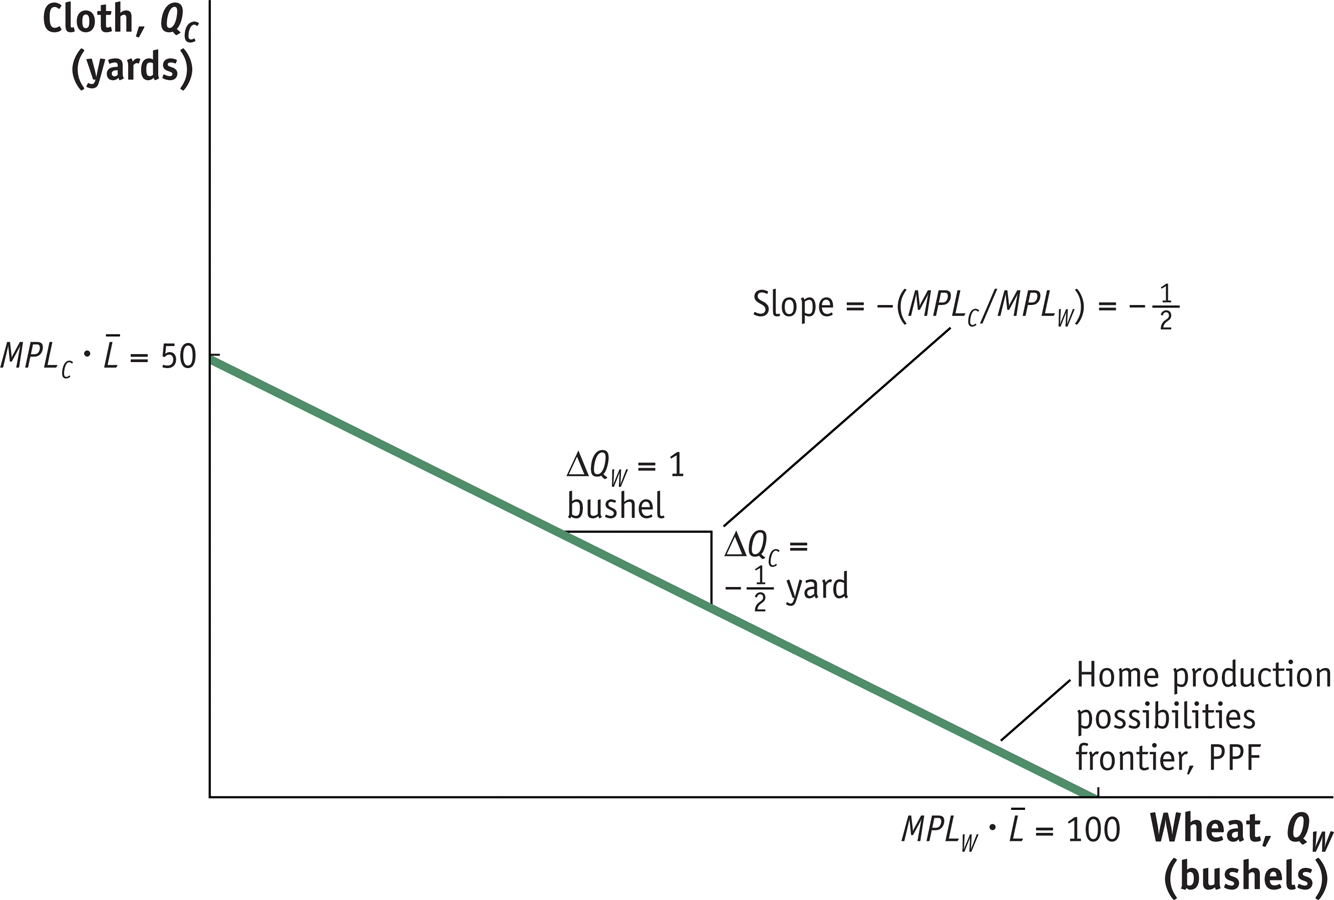
\includegraphics[height=3in,width=4.25in]{Feenstra_Essentials2e_fig_02_01.jpg}
\end{frame}

%%%%%%%%%%%%%%%%%%%%%%%%%%%%%%%%%%%%%%%%%%%%%%%%%%%%%%%%%%%%%%%%%%%%%%%%%%%%%%%%%%%%%%%%%%%%%%%%
%%%%%%%%%%%%%%%%%%%%%%%%%%%%%%%%%%%%%%%%%%%%%%%%%%%%%%%%%%%%%%%%%%%%%%%%%%%%%%%%%%%%%%%%%%%%%%%%


\begin{frame}[t]
\frametitle{Relative Prices}
\begin{itemize}
\item Recall from Chapter 3 Mankiw, profit maximization implies
\begin{eqnarray*}
P \times MPL = W
\end{eqnarray*}
\item In the Ricardian model, workers are free to move and work in the sector paying the highest wages.
\bigskip
\item Thus wages in Cloth sector must equal wages in Wheat sector.
\begin{eqnarray*}
P_w \times MPL_w = W = P_c \times MPL_c\\
\\
\frac{P_w}{P_c} = \frac{MPL_c}{MPL_w} = \frac{2}{4}
\end{eqnarray*}
\medskip
\item The relative price of wheat $=$ the opportunity cost of wheat!
\end{itemize}
\bigskip
\end{frame}

%%%%%%%%%%%%%%%%%%%%%%%%%%%%%%%%%%%%%%%%%%%%%%%%%%%%%%%%%%%%%%%%%%%%%%%%%%%%%%%%%%%%%%%%%%%%%%%%
%%%%%%%%%%%%%%%%%%%%%%%%%%%%%%%%%%%%%%%%%%%%%%%%%%%%%%%%%%%%%%%%%%%%%%%%%%%%%%%%%%%%%%%%%%%%%%%%


\begin{frame}[t]
\frametitle{Equilibrium: Marginal Cost = Marginal Benefit}
\vspace{.2cm}
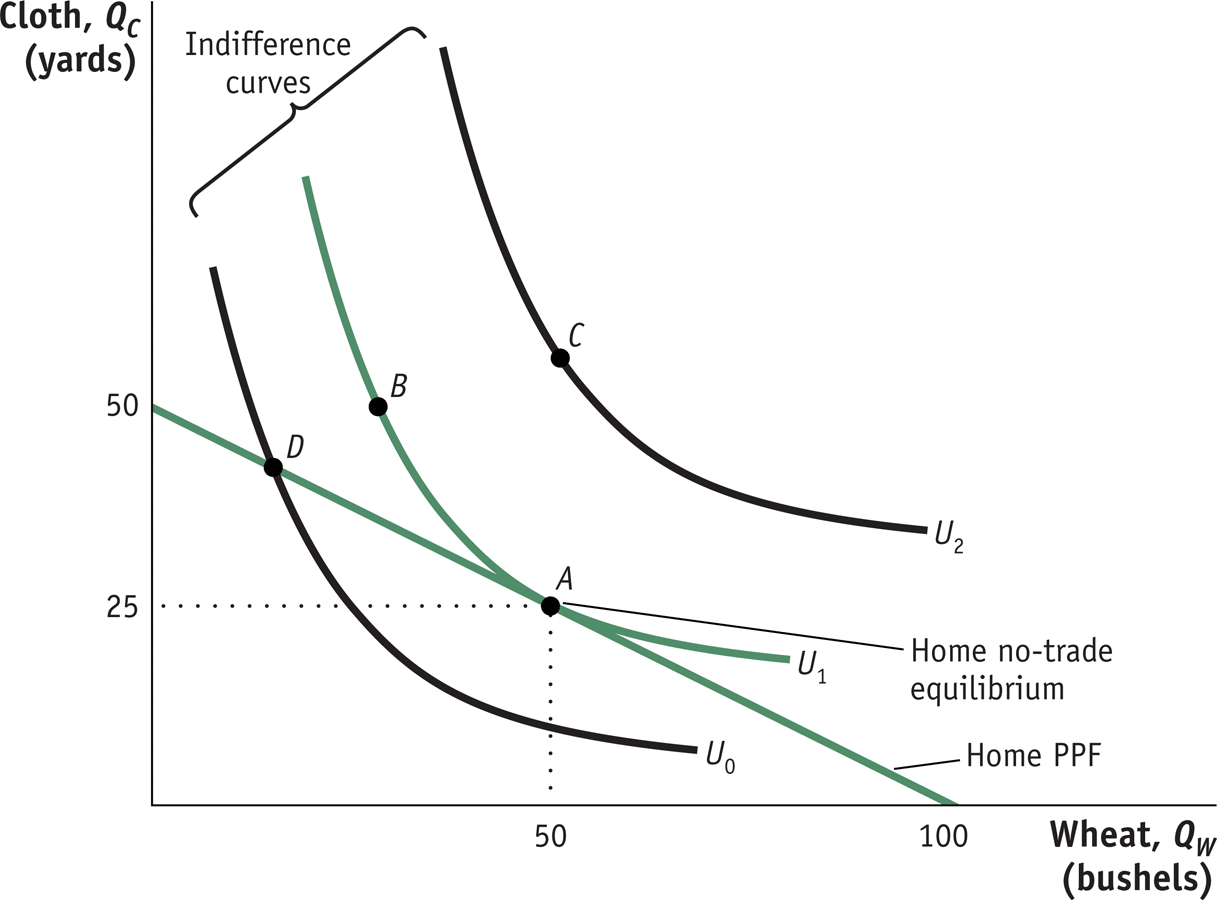
\includegraphics[height=3in,width=4.25in]{Feenstra_Essentials2e_fig_02_02.jpg}
\end{frame}

%%%%%%%%%%%%%%%%%%%%%%%%%%%%%%%%%%%%%%%%%%%%%%%%%%%%%%%%%%%%%%%%%%%%%%%%%%%%%%%%%%%%%%%%%%%%%%%%
%%%%%%%%%%%%%%%%%%%%%%%%%%%%%%%%%%%%%%%%%%%%%%%%%%%%%%%%%%%%%%%%%%%%%%%%%%%%%%%%%%%%%%%%%%%%%%%%


\begin{frame}[t]
\frametitle{Where we are going next\ldots}
\bigskip
\begin{itemize}
\item Pattern of trade.
\bigskip
\item Prices at which countries are willing to trade internationally.
\bigskip
\item Gains from trade.
\end{itemize}
\end{frame}


%%%%%%%%%%%%%%%%%%%%%%%%%%%%%%%%%%%%%%%%%%%%%%%%%%%%%%%%%%%%%%%%%%%%%%%%%%%%%%%%%%%%%%%%%%%%%%%%
%%%%%%%%%%%%%%%%%%%%%%%%%%%%%%%%%%%%%%%%%%%%%%%%%%%%%%%%%%%%%%%%%%%%%%%%%%%%%%%%%%%%%%%%%%%%%%%%
%\begin{frame}[t]
%\frametitle{Time to Enforce A Contract}
%\begin{center}
%\includegraphics[scale=.15]{sachs_warner.pdf}
%\end{center}
%\end{frame}





%%%%%%%%%%%%%%%%%%%%%%%%%%%%%%%%%%%%%%%%%%%%%%%%%%%%%%%%%%%%%%%%%%%%%%%%%%%%%%%%%%%%%%%%%%%%%%%%
%%%%%%%%%%%%%%%%%%%%%%%%%%%%%%%%%%%%%%%%%%%%%%%%%%%%%%%%%%%%%%%%%%%%%%%%%%%%%%%%%%%%%%%%%%%%%%%%


%\begin{frame}[t]
%\frametitle{Credibility or Lack thereof}
%\bigskip
%\begin{itemize}
%\item Policy credibility are very important.
%\bigskip
%\item Good institutions allow governments to commit credibly to good policies help reduce risks and allow businesses to plan with confidence.
%\begin{itemize}
%\medskip
%\item Also known as \textbf{time consistency.}
%\end{itemize}
%\end{itemize}
%\end{frame}
%
%%%%%%%%%%%%%%%%%%%%%%%%%%%%%%%%%%%%%%%%%%%%%%%%%%%%%%%%%%%%%%%%%%%%%%%%%%%%%%%%%%%%%%%%%%%%%%%%%
%%%%%%%%%%%%%%%%%%%%%%%%%%%%%%%%%%%%%%%%%%%%%%%%%%%%%%%%%%%%%%%%%%%%%%%%%%%%%%%%%%%%%%%%%%%%%%%%%
%
%\begin{frame}[t]
%\frametitle{Example of a Time Inconsistent Policy}
%\bigskip
%\begin{itemize}
%\item NATO forces in Western Europe were outnumbered by the Soviet army.
%\bigskip
%\item U.S. announced that it will use the nuclear weapons if the Soviet army
%reached the Rhine.
%\bigskip
%\item But, once the Soviet army breaks through the Fulda Gap, will a U.S. president sacrifice New York or Boston to save Paris?
%\bigskip
%\item A \textbf{time inconsistent policy} is where statments/policies today will not be necessarily followed through in the future when it comes time to do so.
%\bigskip
%\item Similar issues in the taxation of capital...
%\end{itemize}
%\end{frame}
%
%%%%%%%%%%%%%%%%%%%%%%%%%%%%%%%%%%%%%%%%%%%%%%%%%%%%%%%%%%%%%%%%%%%%%%%%%%%%%%%%%%%%%%%%%%%%%%%%%
%%%%%%%%%%%%%%%%%%%%%%%%%%%%%%%%%%%%%%%%%%%%%%%%%%%%%%%%%%%%%%%%%%%%%%%%%%%%%%%%%%%%%%%%%%%%%%%%%
%
%\begin{frame}[t]
%\frametitle{Example of a Time Consistent Policy}
%\bigskip
%\begin{itemize}
%\item PAYGO budget rule in the US Budget Enforcement Act of 1990.
%\begin{itemize}
%\medskip
%\item Tax cuts or entitlement and other mandatory spending increases must be paid for by a tax increase or a cut in mandatory spending.
%\bigskip
%\item If not, automatic spending cuts occur to make this happen, aka ``sequestration.''
%\bigskip
%\item To overcome sequestration, there must 60 votes in the Senate. Hard to do.
%\end{itemize}
%\bigskip
%\item Idea here is commit to a rule that is hard to undo in the future
%\begin{itemize}
%\medskip
%\item Previous example: Rumors of computer program that would automatically nuke the Soviet Union if certain events happen.
%\end{itemize}
%\end{itemize}
%\end{frame}

%\begin{frame}[t]
%\frametitle{Theory: The Parts}
%\includegraphics[height=3in,width=4.25in]{output_diagram_v3}
%\end{frame}
%
%
%%%%%%%%%%%%%%%%%%%%%%%%%%%%%%%%%%%%%%%%%%%%%%%%%%%%%%%%%%%%%%%%%%%%%%%%%%%%%%%%%%%%%%%%%%%%%%%%%
%%%%%%%%%%%%%%%%%%%%%%%%%%%%%%%%%%%%%%%%%%%%%%%%%%%%%%%%%%%%%%%%%%%%%%%%%%%%%%%%%%%%%%%%%%%%%%%%%
%
%
%\begin{frame}[t]
%\frametitle{Argentina}
%\begin{center}
%\includegraphics[scale=.33]{arg1960.pdf}
%\end{center}
%\end{frame}
%%%%%%%%%%%%%%%%%%%%%%%%%%%%%%%%%%%%%%%%%%%%%%%%%%%%%%%%%%%%%%%%%%%%%%%%%%%%%%%%%%%%%%%%%%%%%%%%%
%%%%%%%%%%%%%%%%%%%%%%%%%%%%%%%%%%%%%%%%%%%%%%%%%%%%%%%%%%%%%%%%%%%%%%%%%%%%%%%%%%%%%%%%%%%%%%%%%
%
%\begin{frame}[t]
%\frametitle{Argentina in the 1990's}
%\bigskip
%\begin{itemize}
%\item Argentina:
%\begin{itemize}
%\medskip
%\item Facing inflation over 1000\%, the government
%announced in 1991 that citizens could use
%either dollars or local currency and pegged
%the peso to the dollar. This helped, for a while \ldots \\
%\medskip
%A decade later, the
%government converted all dollar assets into
%pesos (�pesification�) and devalued by 75\%.
%\end{itemize}
%\end{itemize}
%\end{frame}
%
%%%%%%%%%%%%%%%%%%%%%%%%%%%%%%%%%%%%%%%%%%%%%%%%%%%%%%%%%%%%%%%%%%%%%%%%%%%%%%%%%%%%%%%%%%%%%%%%%
%%%%%%%%%%%%%%%%%%%%%%%%%%%%%%%%%%%%%%%%%%%%%%%%%%%%%%%%%%%%%%%%%%%%%%%%%%%%%%%%%%%%%%%%%%%%%%%%%
%
%
%\begin{frame}[t]
%\frametitle{What Happened?}
%\bigskip
%\begin{itemize}
%\item Pegging the Peso meant the government could not finance government debt by printing money.
%\bigskip
%\item This requires\ldots fiscal discipline!
%\begin{itemize}
%\medskip
%\item Provincial governments
%\medskip
%\item Federal government
%\end{itemize}
%\bigskip
%\item Short answer: It did not happen
%\bigskip
%\item Does this sound familiar? Monetary arrangement with good benefits requires fiscal discipline that the government can not keep.\\
%    \medskip
%    Think gyros \ldots
%\end{itemize}
%\end{frame}
%
%%%%%%%%%%%%%%%%%%%%%%%%%%%%%%%%%%%%%%%%%%%%%%%%%%%%%%%%%%%%%%%%%%%%%%%%%%%%%%%%%%%%%%%%%%%%%%%%%
%%%%%%%%%%%%%%%%%%%%%%%%%%%%%%%%%%%%%%%%%%%%%%%%%%%%%%%%%%%%%%%%%%%%%%%%%%%%%%%%%%%%%%%%%%%%%%%%%
%
%\begin{frame}[t]
%\frametitle{Argentina Today}
%\bigskip
%\begin{itemize}
%\item Late 2008: Argentina nationalized private pension funds
%\begin{itemize}
%\medskip
%\item Goal was to ``protect'' the money from the global financial crisis.
%\end{itemize}
%\bigskip
%\item January 2009: President fires central bank president and seizes monetary reserves
%\begin{itemize}
%\medskip
%\item Goal was to payoff foreign creditors but preserve treasury revenues
%\medskip
%\item Treasury revenues for paying off constituencies ahead of upcoming election
%\end{itemize}
%\bigskip
%\item Good governance?
%\end{itemize}
%\end{frame}
%
%%%%%%%%%%%%%%%%%%%%%%%%%%%%%%%%%%%%%%%%%%%%%%%%%%%%%%%%%%%%%%%%%%%%%%%%%%%%%%%%%%%%%%%%%%%%%%%%%
%%%%%%%%%%%%%%%%%%%%%%%%%%%%%%%%%%%%%%%%%%%%%%%%%%%%%%%%%%%%%%%%%%%%%%%%%%%%%%%%%%%%%%%%%%%%%%%%%
%\begin{frame}[t]
%\frametitle{Argentina and Ireland}
%\begin{center}
%\includegraphics[scale=.33]{arg_irl.pdf}
%\end{center}
%\end{frame}
%
%%%%%%%%%%%%%%%%%%%%%%%%%%%%%%%%%%%%%%%%%%%%%%%%%%%%%%%%%%%%%%%%%%%%%%%%%%%%%%%%%%%%%%%%%%%%%%%%%
%%%%%%%%%%%%%%%%%%%%%%%%%%%%%%%%%%%%%%%%%%%%%%%%%%%%%%%%%%%%%%%%%%%%%%%%%%%%%%%%%%%%%%%%%%%%%%%%%
%\begin{frame}[t]
%\frametitle{Ireland}
%\bigskip
%\begin{itemize}
%\item EU membership and aid recipient
%\bigskip
%\item Fiscal discipline ($>$1987)
%\begin{itemize}
%\medskip
%\item Government hiring frozen
%\medskip
%\item Personal and corporate tax rates slashed
%\medskip
%\item Government budget balanced
%\end{itemize}
%\bigskip
%\item Very attractive conditions for foreign firms
%\begin{itemize}
%\medskip
%\item Lowest corporate tax rates in OECD
%\end{itemize}
%\bigskip
%\item Facing pressure today \ldots but past history suggests they have ability to make the ``right'' decisions.
%\end{itemize}
%\end{frame}
%
%%%%%%%%%%%%%%%%%%%%%%%%%%%%%%%%%%%%%%%%%%%%%%%%%%%%%%%%%%%%%%%%%%%%%%%%%%%%%%%%%%%%%%%%%%%%%%%%%
%%%%%%%%%%%%%%%%%%%%%%%%%%%%%%%%%%%%%%%%%%%%%%%%%%%%%%%%%%%%%%%%%%%%%%%%%%%%%%%%%%%%%%%%%%%%%%%%%
%
%%%%%%%%%%%%%%%%%%%%%%%%%%%%%%%%%%%%%%%%%%%%%%%%%%%%%%%%%%%%%%%%%%%%%%%%%%%%%%%%%%%%%%%%%%%%%%%%%
%%%%%%%%%%%%%%%%%%%%%%%%%%%%%%%%%%%%%%%%%%%%%%%%%%%%%%%%%%%%%%%%%%%%%%%%%%%%%%%%%%%%%%%%%%%%%%%%%
%
%\begin{frame}[t]
%\frametitle{Recap}
%\bigskip
%\begin{itemize}
%\item Good institutions
%\begin{itemize}
%\medskip
%\item Put capital and labor to efficient use
%\end{itemize}
%\bigskip
%\item Examples
%\begin{itemize}
%\medskip
%\item Rule of law
%\medskip
%\item Property rights
%\medskip
%\item Competitive markets
%\end{itemize}
%\bigskip
%\item Evidence suggests countries with poor economic performance lack these institutions.
%\end{itemize}
%\end{frame}

\end{document} 